\chapter{\label{CH:challenges}Challenges in data reduction. Etalon Cavity Map.}

\section{\label{ch3: cavity map}Cavity map retrieval from flat-field observations}



\subsection{One device, two configurations}

file:///home/pablo/Downloads/s10509-023-04212-3.pdf



\subsubsection{Collimated configuration}

Collimated mounts are characterized by having the etalon located at the pupil plane and therefore receive a collimated beam from each point of the observed object. In this setup, light coming from any point of the object will fall upon the same area of the etalon. Consequently, any local defects on the etalon crystals or on the plates' parallelism is averaged all over the clear aperture, thus making the optical quality constant along the FoV. However, the angle of incidence of the light beam varies along the FoV, thus shifting the transmission profile.  

 The transmission profile for an ideal collimated etalon tuned at wavelength $\lambda _ s$ takes the following form:
\begin{equation}
\Psi ^{\lambda _ s} (\lambda, \theta) = \frac{1}{1 + F \sin ^2 a_s (\lambda,\theta) },
\end{equation}
where
\begin{equation}
a_s (\lambda, \theta) =\frac{2  \pi}{\lambda} nd\cos \theta  \ ,
\label{eq: a-def}
\end{equation}
with the subscript $s$ indicating that the etalon is tuned at the wavelength $\lambda_s$.

The shape of the transmission profile depends on its physical properties. Firstly, the width of the resonance peaks is determined by the parameter $F$, $F \equiv 4R (1 - R )^{-2}$, which depends exclusively on the reflectivity $R$ of its mirrors. Secondly, the spectral behavior of the transmission profile is governed by $a_s(\lambda,\theta)$, which is a function of the refractive index of the etalon cavity, $n$; the distance between mirrors, $d$; and the angle of the incident beam, $\theta$. 

Local defects in the collimated configuration are averaged out, which means that $d$ and $n$ respectively represent the mean values of the thickness and refractive index across the clear aperture of the FPI. Yet, they produce a broadening of the transmission profile and worsen the optical quality of the instrument. The differing angles of incidence over the FoV produce shifts of the transmission that vary quadratically with $\theta$.

\subsubsection{\label{susec: Tele-perfe}Telecentric configuration}

In the telecentric configuration, the etalon is placed very close to an intermediate focal plane, while the pupil is focused at infinity. This way, the etalon is illuminated by cones of rays that are parallel to each other and reach different sections of the interferometer. Local inhomogeneities (defects or cavities) on the etalon produce differences in the transmission profile across the FoV, which are directly mapped into the image plane. This means that the optical response and the transmission profile shift locally on the image sensor. 

The transmission profile of the etalon tuned at a wavelength $\lambda _s $ is, in this case, given by \citep{franIV}:
\begin{equation}
\Psi ^{\lambda _ s} (\lambda) =  \mathfrak{Re}\left[E(a_s (\lambda, n, d, \theta), b) \right] ^2 + \mathfrak{Im}\left[E(a_s(\lambda, n, d, \theta), b) \right] ^2 ,
\label{Eqn: Tel_first}
\end{equation}
with $E(a,b)$ being:
\begin{multline}
E(a, b) = 2 \sqrt{\tau}\ \Biggl\{ \int_0^1 \frac{\varrho \cos \left(a\left[1-b \varrho^2\right]\right)}{1+F \sin ^2\left(a\left[1-b \varrho^2\right]\right)} \mathrm{d} \varrho \ + \\
\mathrm{i} \frac{1+R}{1-R} \int_0^1 \frac{\varrho \sin \left(a\left[1-b \varrho^2\right]\right)}{1+F+ \sin ^2\left(a\left[1-b \varrho^2\right]\right)} \mathrm{d} \varrho\Biggr\} ,
\end{multline}
where $\tau$ is the transmission factor of the etalon at normal incidence, $\varrho$ is the radial coordinate of the pupil normalized to the pupil radius of the instrument, $a$ is defined by Eq. \eqref{eq: a-def} and $b$ is given by
\begin{equation}
b = \frac{1}{8 (nf\#) ^2}.
\end{equation}

This parameter accounts for the contribution of the focal ratio, $f\#$, and has an impact on the spectral resolution and the apodization of the pupil as seen from the etalon \citep{beckers}. Thus, the resolution is now affected by both $F$ and $f\#$, through the parameters $a$ and $b$.

Contrary to the collimated case, $a$ now has an explicit dependence on the spatial coordinates of the image plane, as $n$ and $d$ change from pixel to pixel. These variations compose the "cavity error" of the etalon and need to be corrected when employing telecentric configurations.

\subsubsection{Telecentric imperfect configuration}
The equations shown in Sect.~\ref{susec: Tele-perfe} are valid whenever the incident cone of rays is perpendicular to the etalon mirrors. We refer to this situation hereinafter as "perfect telecentrism". However, real instruments are likely to present deviations from such an ideal case. These deviations can be caused by an intentional tilt of the etalon to suppress ghost images on the detector \citep{ghosts-etalon}, by an accidental tilted angle of incidence caused by deviations from the ideal paraxial propagation of rays within the instrument, or simply because of misalignment of the optical components. In the three cases, the incident cone of rays is no longer perpendicular to the etalon, and hence, we consider these scenarios to have imperfections in the telecentrism degree. One important consequence of the loss of telecentrism is an asymmetrization of the transmission profile that must be accounted for when modeling the instrument response.

The transmission profile in this case is influenced by the angle of incidence of the chief ray at each point of the clear aperture of the etalon, in addition to the parameters mentioned in the previous sections. Unfortunately, the equations for the transmission profile in these configurations are much more complicated than in the ideal telecentric case, with no analytical solution to the integrals of the transmission profile. The integrals and their corresponding derivatives can only be obtained via numerical methods \citep{franI}. 
\begin{figure}
    \centering
    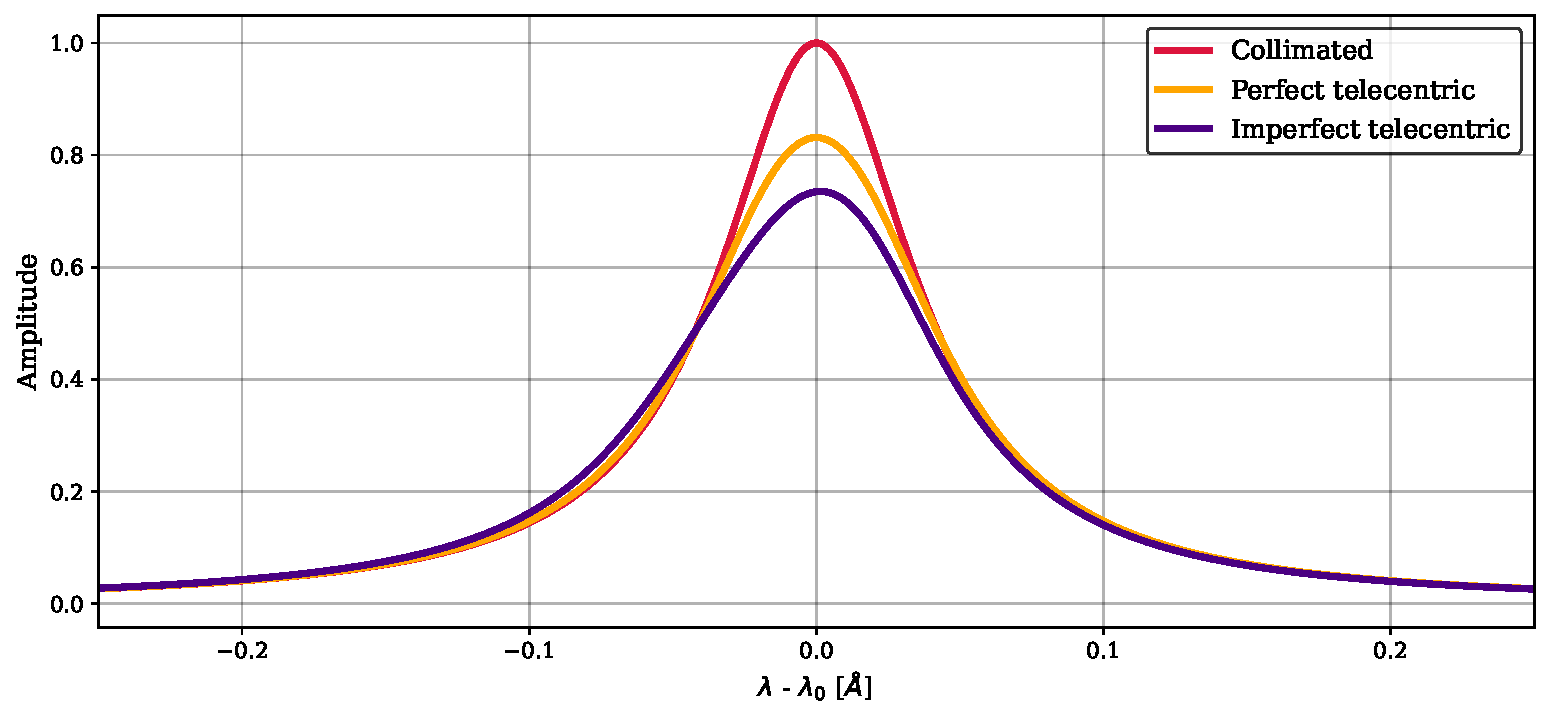
\includegraphics[width = \textwidth]{figures/EtalonPaper/etalon_setups_profiles.pdf}
    \caption{Central peak of the etalon's transmission profile for the three different configurations. The parameters of the etalon are $R = 0.92$, $n = 2.29$, $d = 251 \, \mu \mathrm{m}$, $f\#=56$, $\theta = 0 ^{\circ}$ (collimated and perfect telecentric), and $\Theta = 0.3\,^{\circ}$ (imperfect telecentric)}
    \label{fig_etalon:Profiles-configs}
\end{figure}
Figure \ref{fig_etalon:Profiles-configs} shows the transmission profile corresponding to the three different scenarios we have considered: collimated illumination of the etalon, perfect telecentrism, and imperfect telecentrism. The etalon parameters have been selected to coincide with those of SO/PHI's etalon. In both the collimated and perfect telecentric configurations, a normal incidence  ($\theta = 0$) scenario is shown, whereas in the imperfect telecentric case, we assumed an angle of incidence of the chief ray, $\Theta$, of $0.3^{\circ}$. The parameter $a$ has been adjusted slightly in order to tune the transmission profile at $\lambda _ 0$.

We observed that the telecentric configurations achieve lower peak transmissions than the collimated case. In addition, the telecentric profiles are wider due to the different incidence angles across the illuminating cone of rays. Such a broadening increases with decreasing f-ratios. Lastly, non-normal incidence of the chief ray in the telecentric configuration further widens and shifts ($\sim 4$~m\r{A}
for $\Theta=0.3^\circ$) the profile, making it asymmetrical. 



\section{Sunspot observation simulation.}